\renewcommand{\drawGraduations}[4]{%
    % #1: Start value
    % #2: End value
    % #3: Offset value (for continuity)

    % Centièmes graduations (réduction du nombre de graduations)
    \def\scalefactor{2}

    \foreach \x in {#1,0.1,...,#2} {
        \draw[very thick] (0,\x*\scalefactor) -- (0.6, \x*\scalefactor);
    }

    % Dixièmes graduations
    \foreach \x in {\fpeval{#1},1,...,#2} {
        \draw[very thick] (0,\fpeval{(\x+#4)*\scalefactor}) -- (1.5, \fpeval{(\x+#4)*\scalefactor});
    }

    % Unités graduations et affichage en grand et gras pour les entiers
    \foreach \x in {\fpeval{#1+#4},1,...,\fpeval{#2+0.1}} {
        \pgfmathsetmacro{\write}{(\x + #3) / (10)}
        \pgfmathsetmacro{\value}{((\x + #3)*\scalefactor) / (10)}
        \pgfmathsetmacro{\semivalue}{((\x + #3 + 5*#4)*\scalefactor)  / (10)}
        \pgfmathsetmacro{\semiremainder}{mod(\semivalue,1)}
        \pgfmathsetmacro{\remainder}{mod(\value,1)}
        \ifdim \remainder pt = 0pt
            \node[left, font=\bfseries\LARGE] at (0, \x*\scalefactor) {\num{\fpeval{\write}}};
            %\draw[very thick] (0,\x*\scalefactor+#4) -- (1.5, \x*\scalefactor+#4);
        \fi
        %\ifdim \semiremainder pt = 0pt
        %    \node[left, font=\bfseries\large] at (0, \x*\scalefactor) {\num{\fpeval{\write}}};
        %    %\draw[very thick] (0,\x*\scalefactor+#4) -- (1.5, \x*\scalefactor+#4);
        %\fi
    }

        % Gamification : ajouter des événements aléatoires
        \pgfmathsetmacro{\randomShift}{rnd*4 - 2} % Générer une variation entre -2 et +2
        \pgfmathsetmacro{\eventCount}{int(\fpeval{(5 + \randomShift)/\scalefactor})} % Base 5 événements avec une variation de -2 à +2
        \foreach \i in {1,...,\eventCount} {
        \pgfmathsetmacro{\randY}{random(\fpeval{#1*\scalefactor},\fpeval{(#2 - 3)*\scalefactor})}
        \pgfmathrandominteger{\randheight}{1}{2}
        \pgfmathsetmacro{\randX}{0.5*\bandwidth}
        \pgfmathrandominteger{\eventType}{1}{4}
        \def\eventcolor{yellow}
        \def\eventTextColor{black}
        % Définition des labels selon l'événement
        \ifnum\eventType=1
            \def\eventText{R}%Relancer les dés
            \def\eventcolor{green!85!black}
        \fi
        \ifnum\eventType=2
            \def\eventText{M}%Événement malchanceux}
            \def\eventcolor{red!85!black}
            \def\eventTextColor{white}
        \fi
        \ifnum\eventType=3
            \def\eventText{C}%Événement chanceux}
            \def\eventcolor{green!75!white}
        \fi
        \ifnum\eventType=4
            \def\eventText{D}%Défi}
            \def\eventcolor{orange}
        \fi
        % Dessiner l'événement à une position aléatoire
        \draw[fill=\eventcolor, rounded corners] (\randX, \randY) rectangle ++(2, \fpeval{(\randheight+1)*\scalefactor});

        % Calcul de l'intervalle et placement des labels
        \pgfmathsetmacro{\startY}{\randY}
        \pgfmathsetmacro{\endY}{\randY + \randheight*\scalefactor}
        \foreach \y in {\startY, \fpeval{\startY + 1*\scalefactor}, ..., \endY} {
            \node at (\randX + 1, \y + 0.5*\scalefactor) {\LARGE{\textbf{\color{\eventTextColor}\eventText}}};
        }
    }
    
    % Languette de collage pour lier à la frise suivante
    \draw[thick, fill=gray!30] (0, \bandheight) rectangle (\bandwidth, \bandheight + \languette);
    \node[above, font=\small] at (\bandwidth/2, \bandheight + \languette / 10) {Languette de collage};
}

La frise suivante est à découper. 

Il suffit ensuite de coller les languettes, pour assembler la frise.

\def\scalefactor{2}
Longueur totale : $\num{\fpeval{10 * \scalefactor * 137.5}}$
\newpage

% Définition des constantes
\def\bandwidth{4.5} % Largeur d'une bande en cm
\def\bandheight{25} % Hauteur d'une bande en cm
\def\languette{0.8}
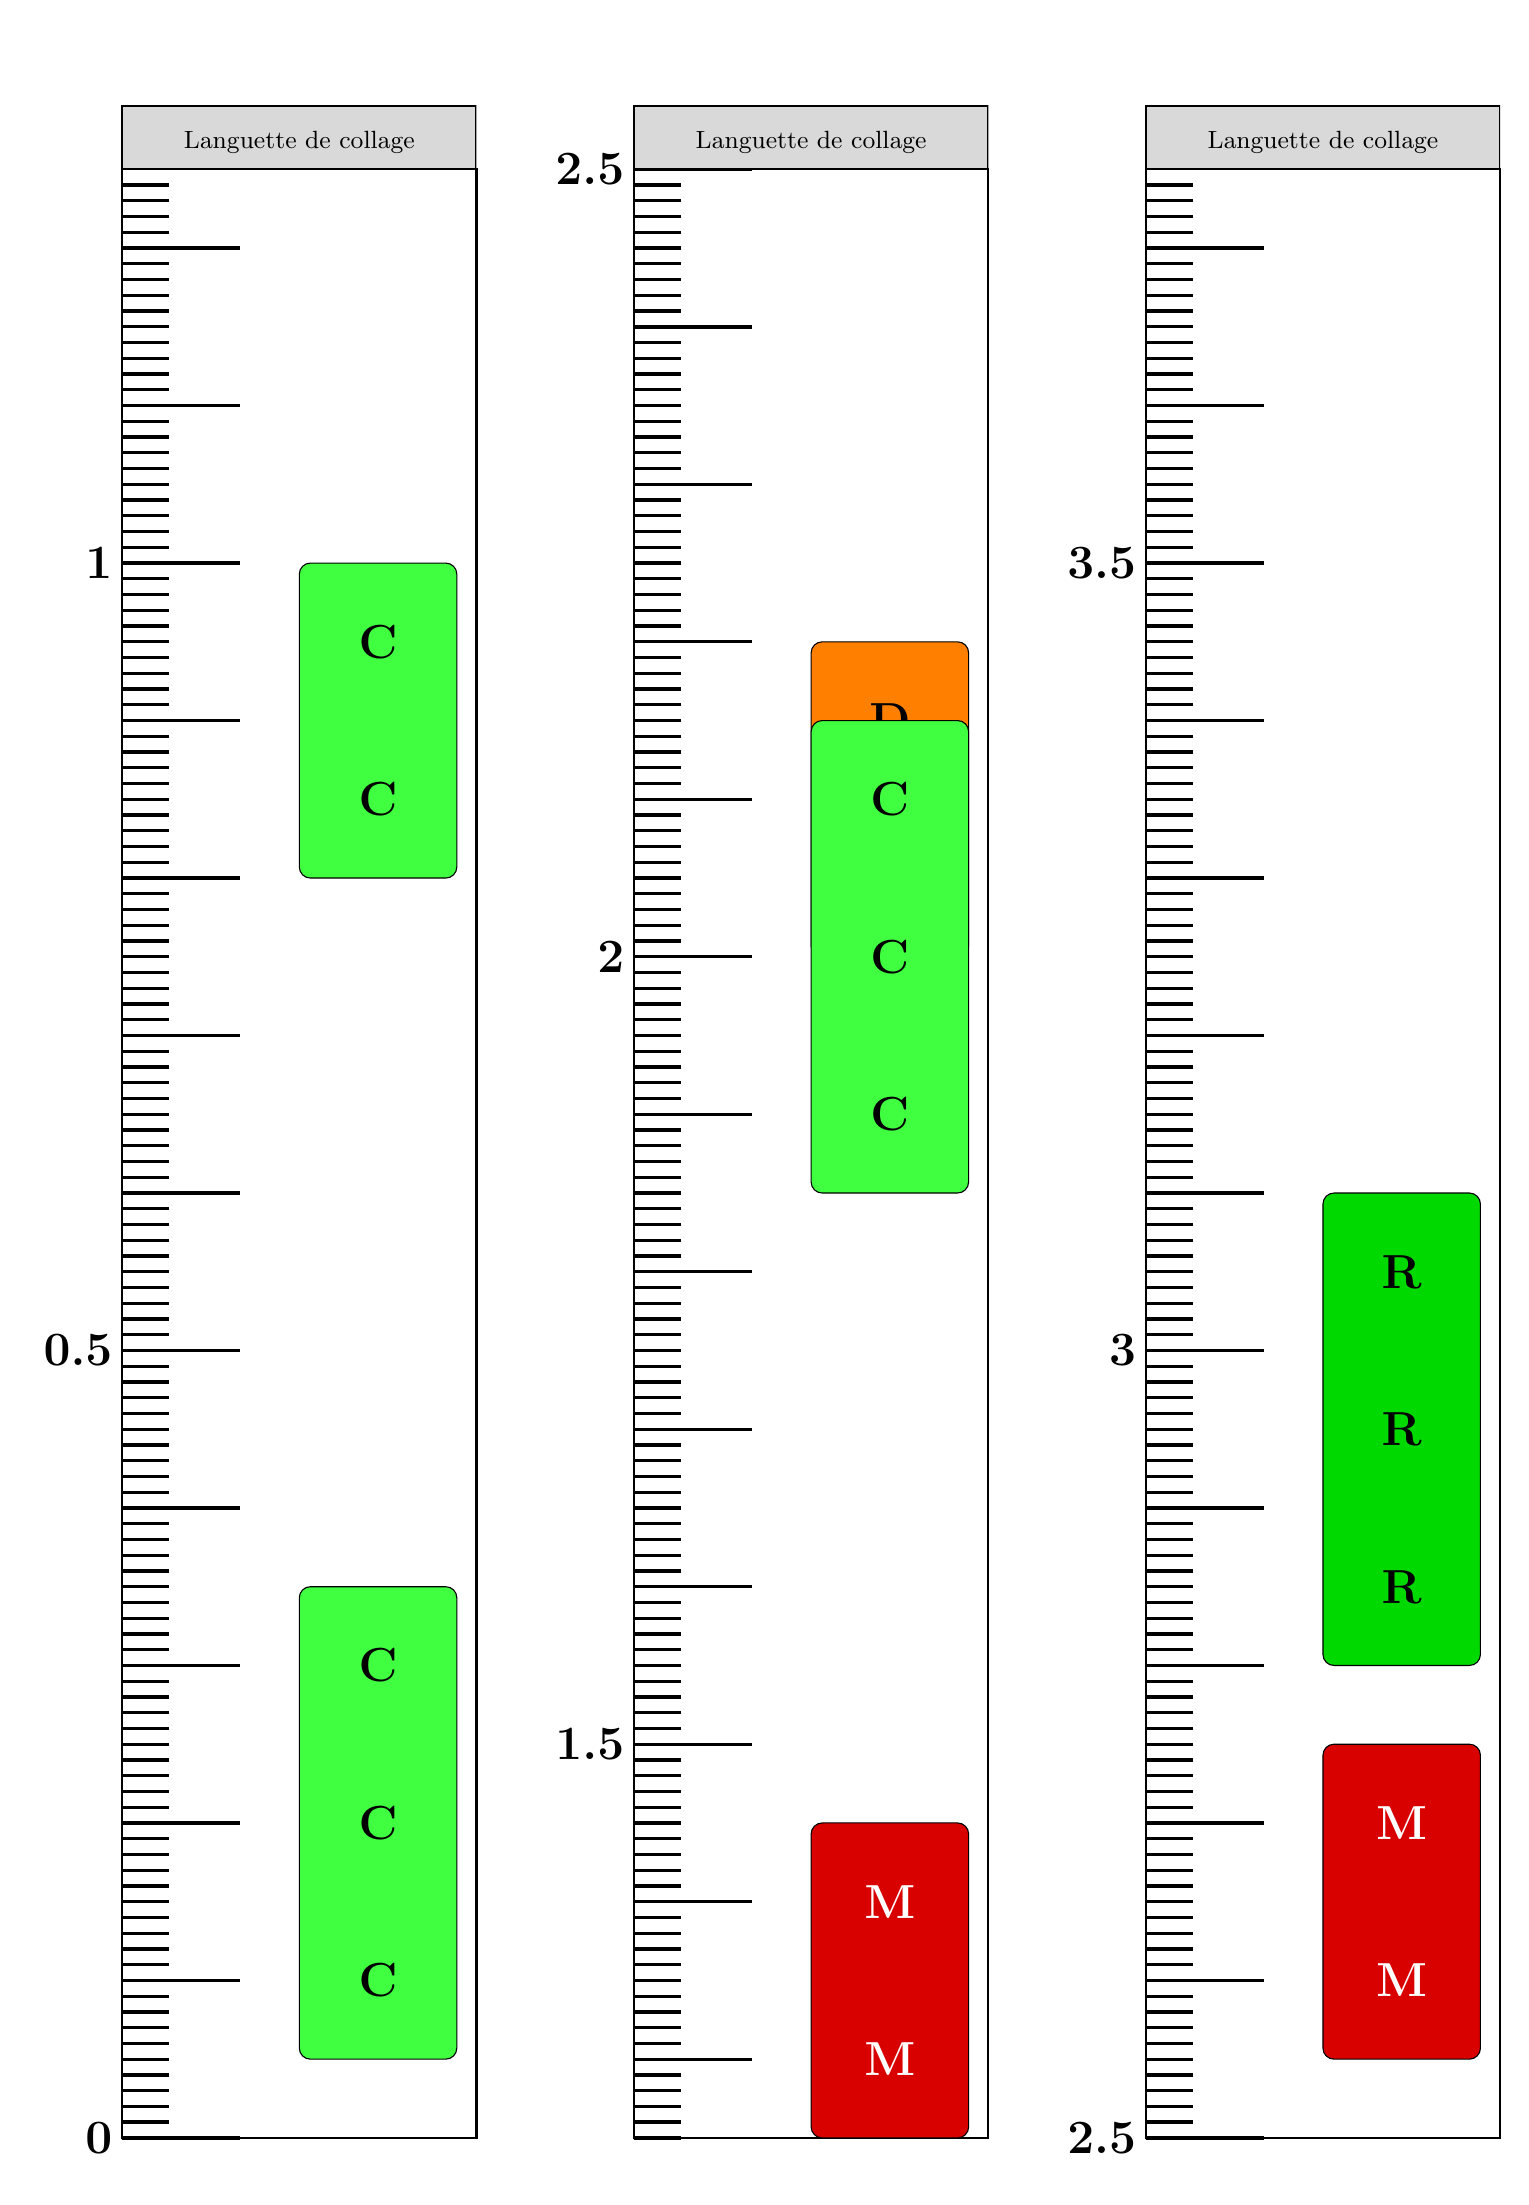
\begin{tikzpicture}[x=1cm, y=1cm,xshift=-1cm]

% Dessin de la première bande
\begin{scope}[shift={(-1,0)}]
    \draw[thick] (0,0) rectangle (\bandwidth, \bandheight);
    \clip (-1.2,-0.5) rectangle (\bandwidth, \bandheight+\languette+1);
    \drawGraduations{0}{12.5}{0}{0}
\end{scope}

% Dessin de la deuxième bande (avec continuité des nombres)
\begin{scope}[shift={(1*\bandwidth + 1,0)}]
    \draw[thick] (0,0) rectangle (\bandwidth, \bandheight);
    \clip (-1.2,-0.5) rectangle (\bandwidth, \bandheight+\languette+1);
    \drawGraduations{0}{12.5}{12.5}{0.5}
\end{scope}

% Dessin de la troisième bande (avec continuité des nombres)
\begin{scope}[shift={(2*\bandwidth + 3,0)}]
    \draw[thick] (0,0) rectangle (\bandwidth, \bandheight);
    \clip (-1.2,-0.5) rectangle (\bandwidth, \bandheight+\languette+1);
    \drawGraduations{0}{12.5}{25}{0}
\end{scope}

\end{tikzpicture}

\newpage

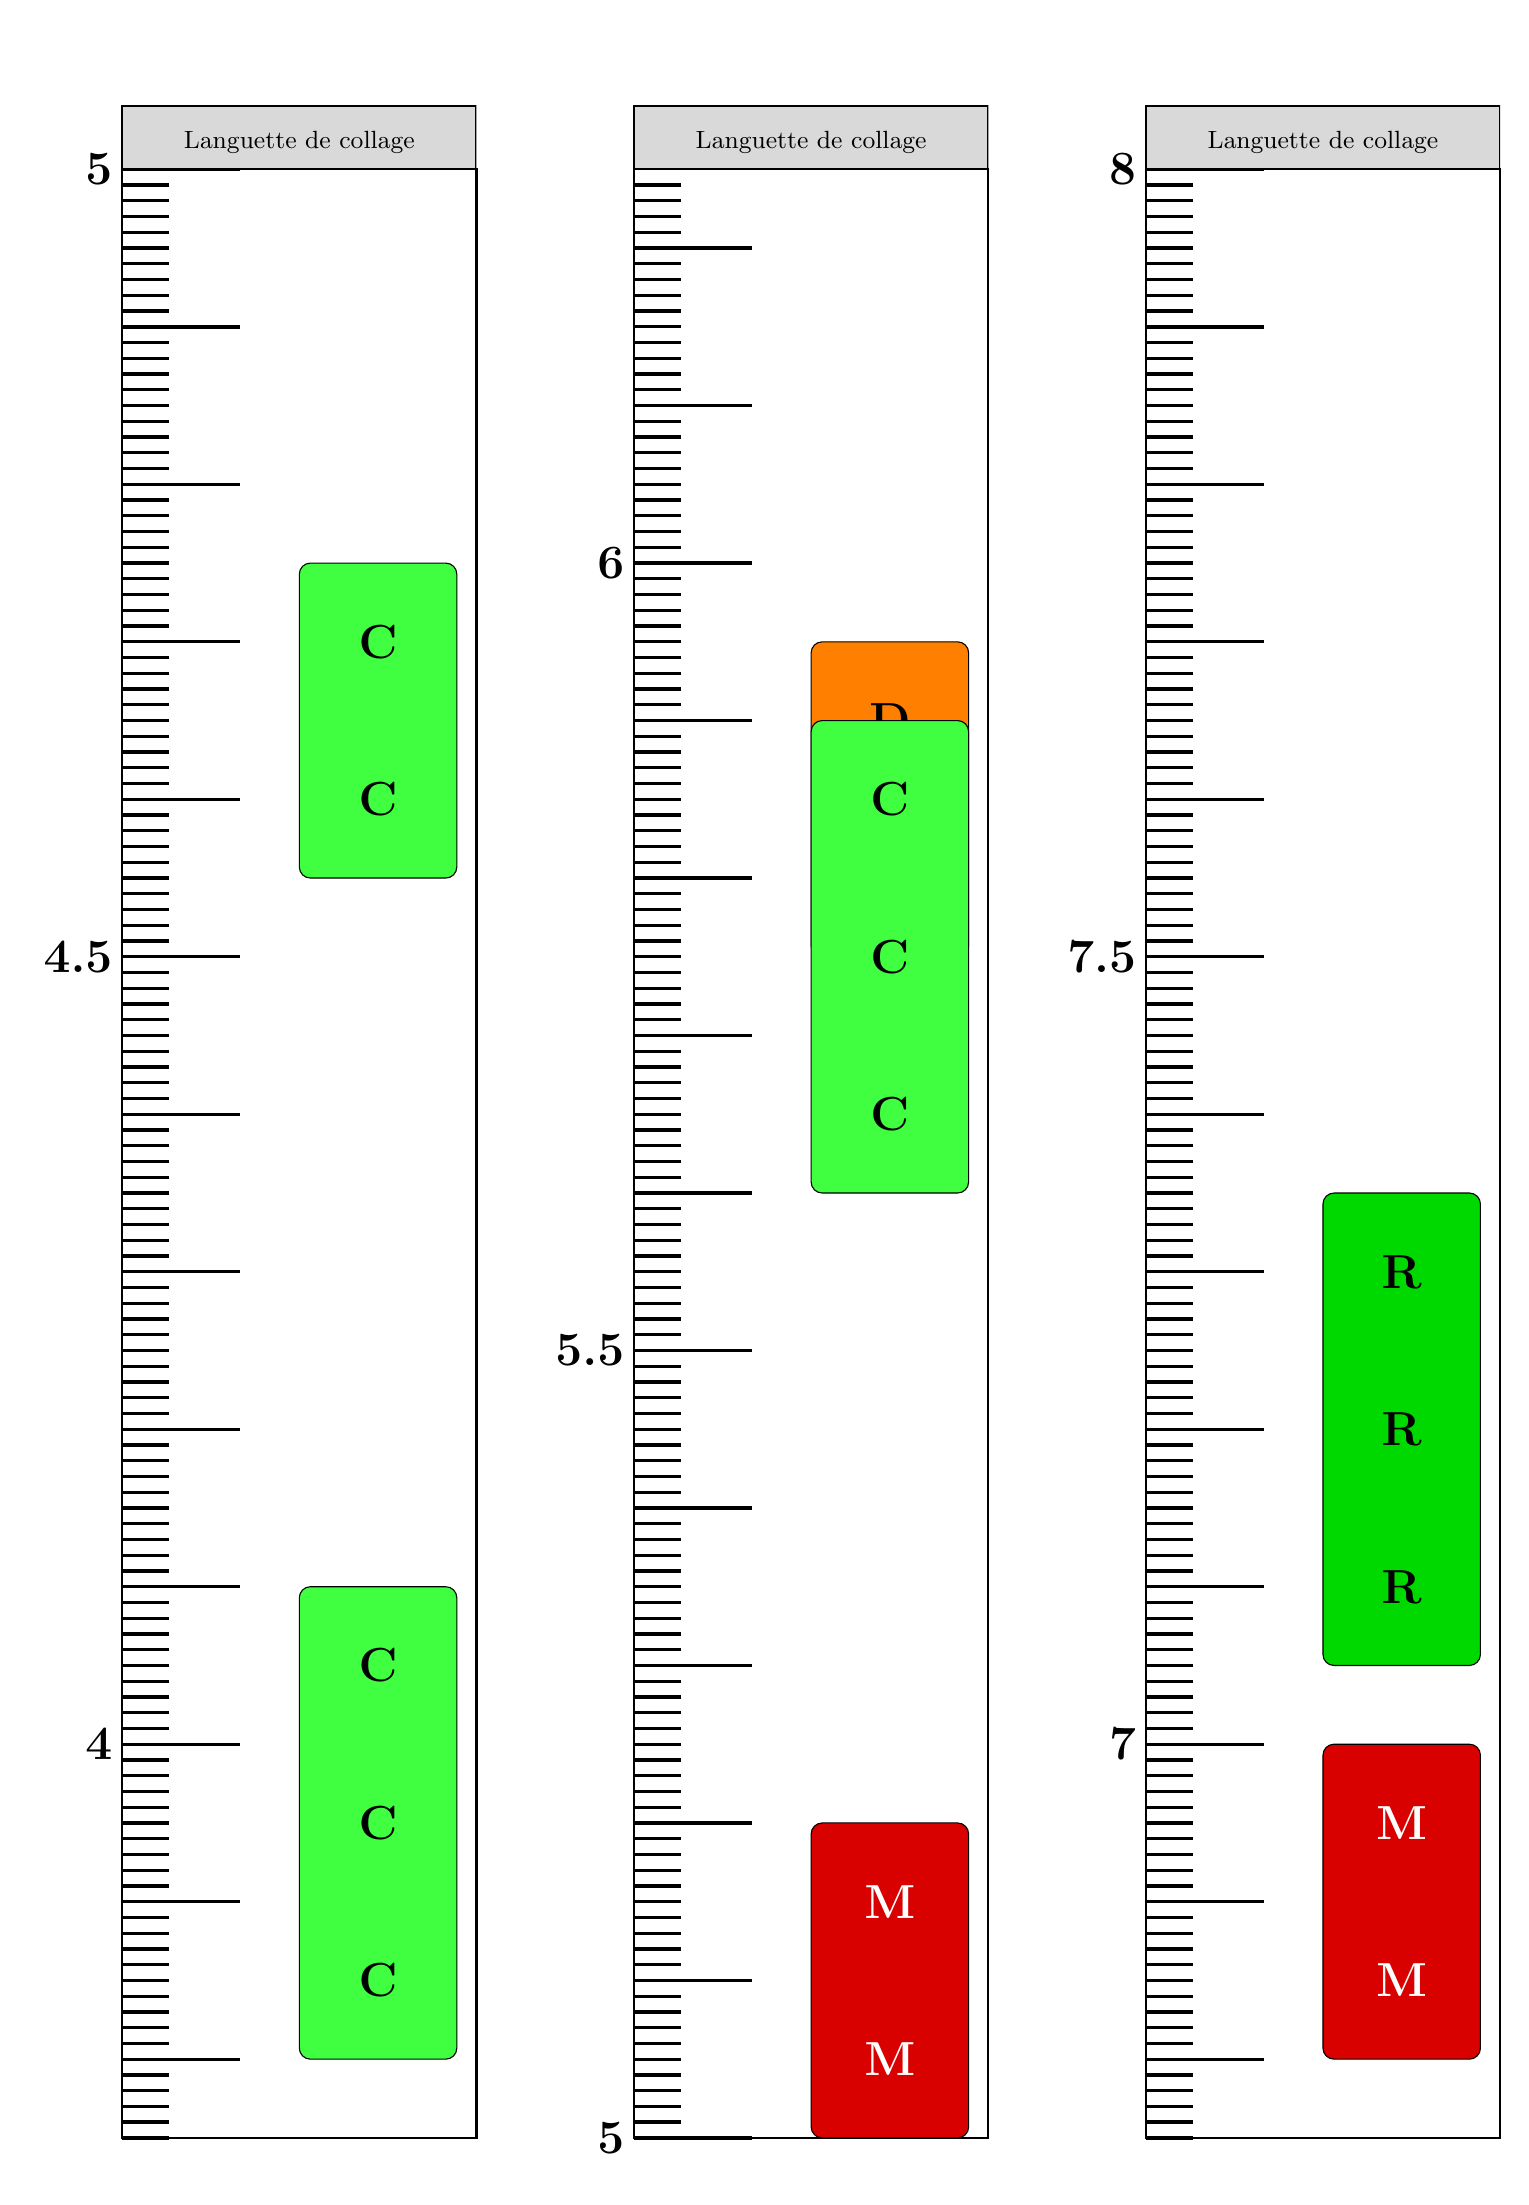
\begin{tikzpicture}[x=1cm, y=1cm,xshift=-1cm]
% Dessin de la première bande
\begin{scope}[shift={(-1,0)}]
    \draw[thick] (0,0) rectangle (\bandwidth, \bandheight);
    \clip (-1.2,-0.5) rectangle (\bandwidth, \bandheight+\languette+1);
    \drawGraduations{0}{12.5}{37.5}{0.5}
\end{scope}

% Dessin de la deuxième bande (avec continuité des nombres)
\begin{scope}[shift={(1*\bandwidth + 1,0)}]
    \draw[thick] (0,0) rectangle (\bandwidth, \bandheight);
    \clip (-1.2,-0.5) rectangle (\bandwidth, \bandheight+\languette+1);
    \drawGraduations{0}{12.5}{50}{0}
\end{scope}

% Dessin de la troisième bande (avec continuité des nombres)
\begin{scope}[shift={(2*\bandwidth + 3,0)}]
    \draw[thick] (0,0) rectangle (\bandwidth, \bandheight);
    \clip (-1.2,-0.5) rectangle (\bandwidth, \bandheight+\languette+1);
    \drawGraduations{0}{12.5}{67.5}{0.5}
\end{scope}

\end{tikzpicture}

\newpage

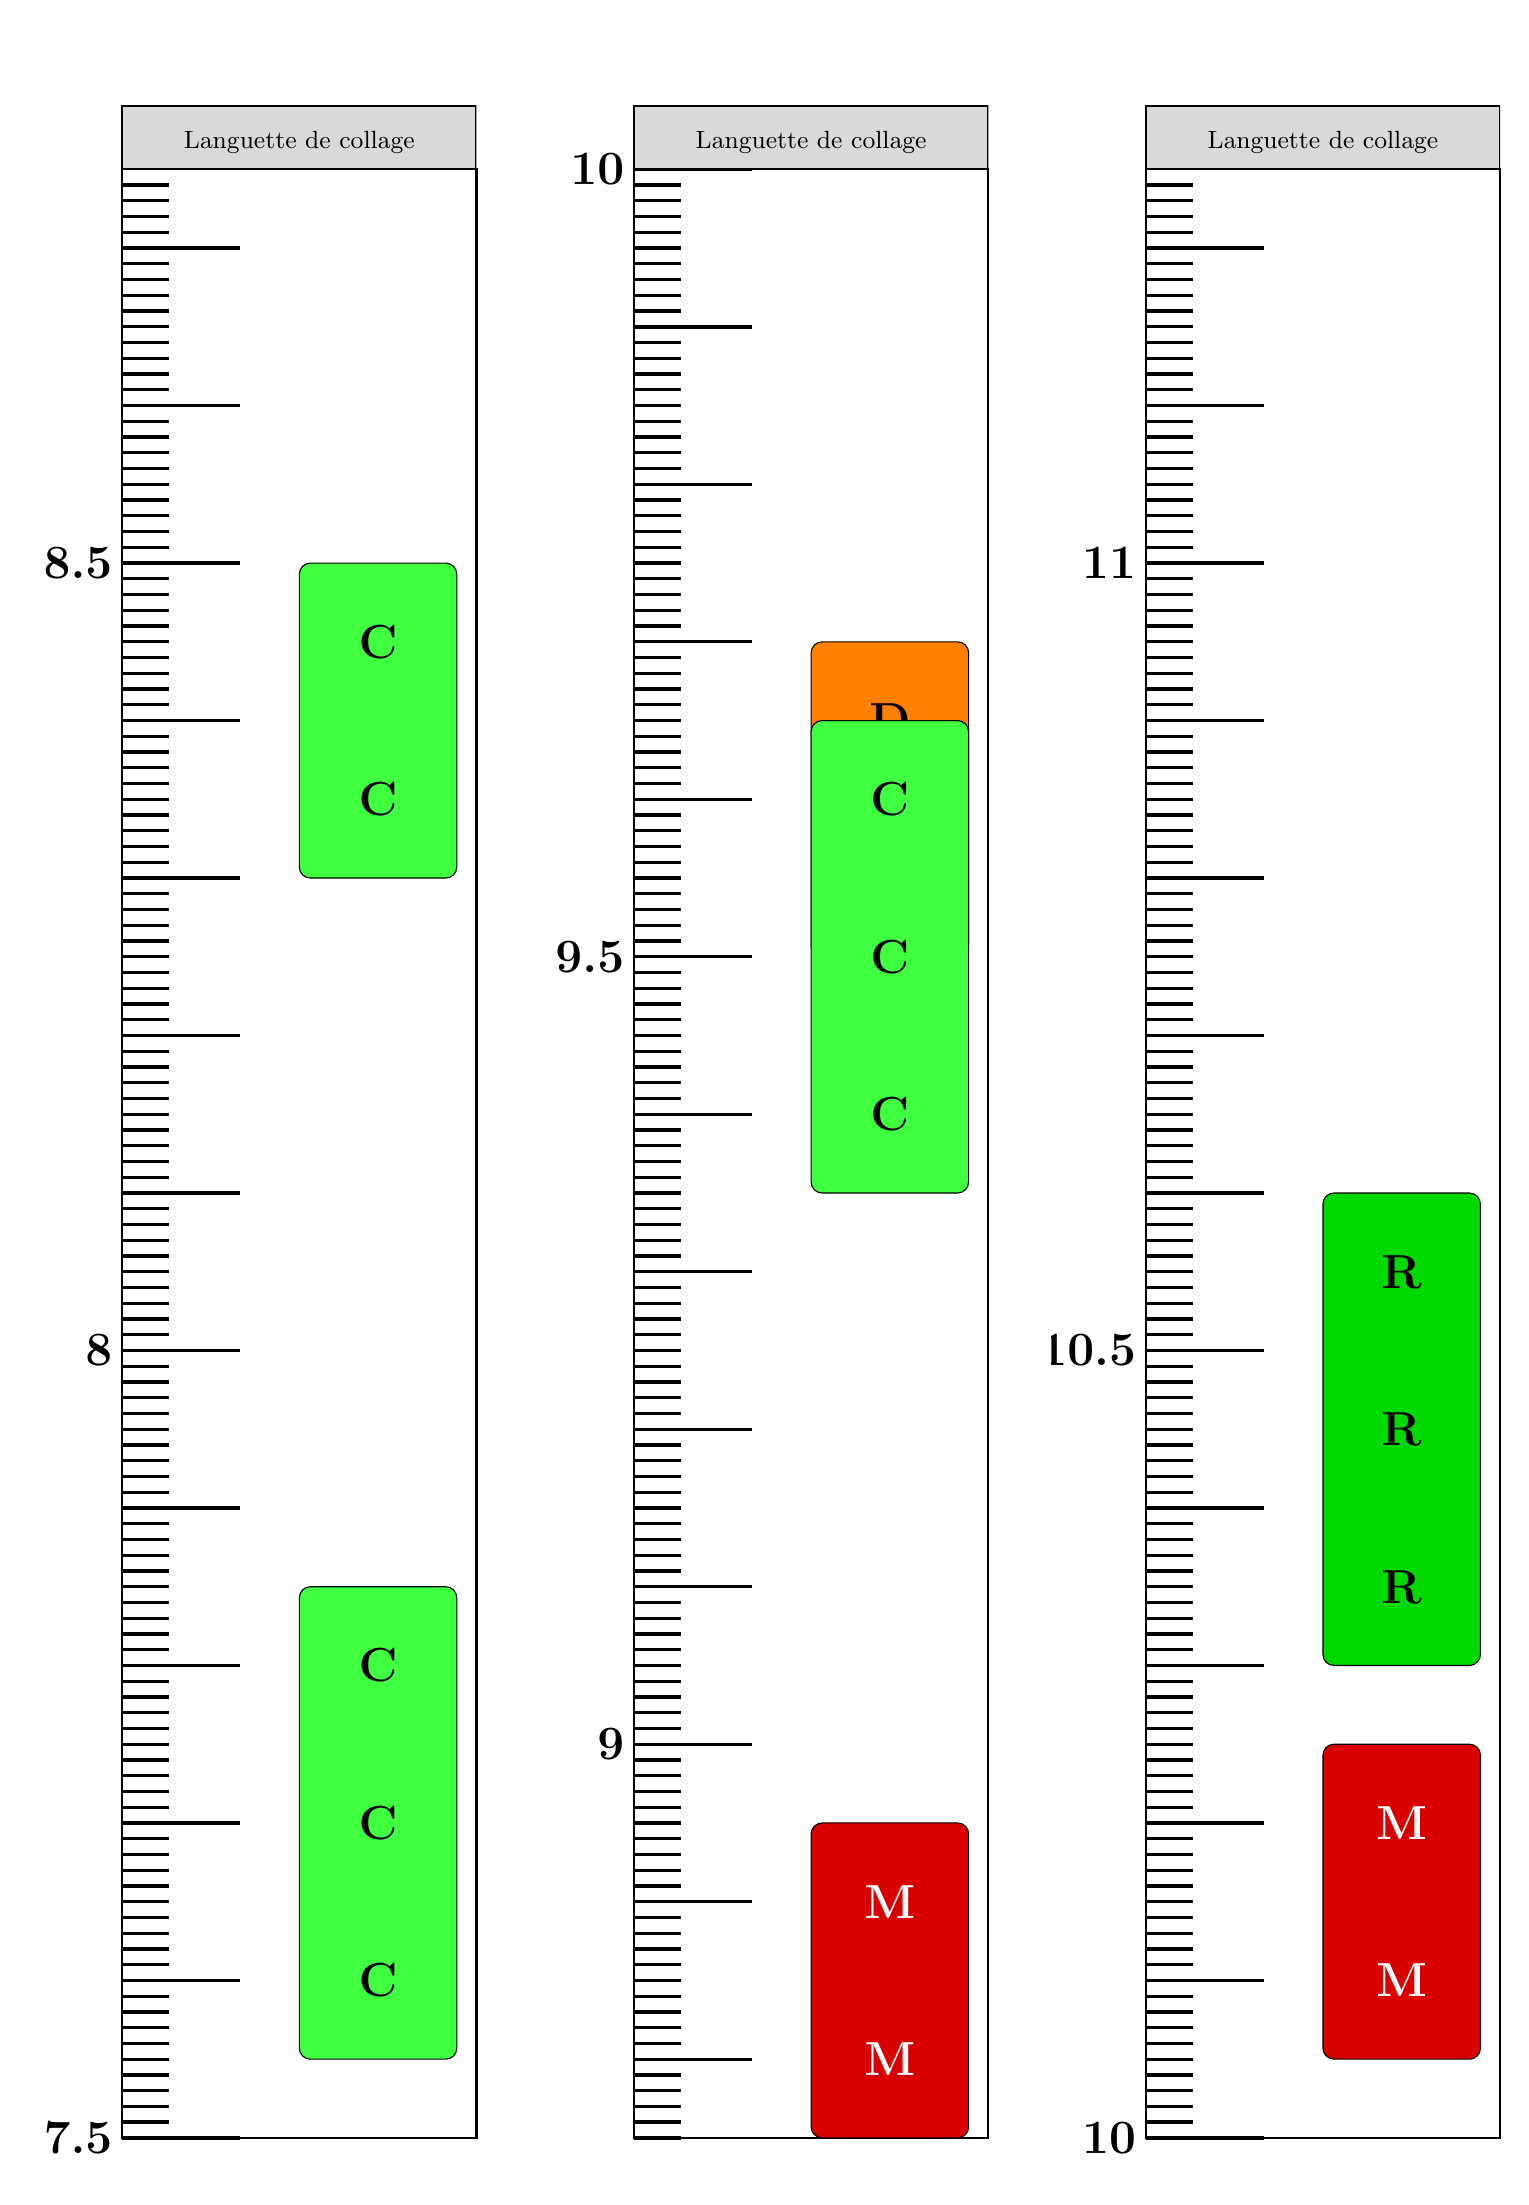
\begin{tikzpicture}[x=1cm, y=1cm,xshift=-1cm]

% Dessin de la première bande
\begin{scope}[shift={(-1,0)}]
    \draw[thick] (0,0) rectangle (\bandwidth, \bandheight);
    \clip (-1.2,-0.5) rectangle (\bandwidth, \bandheight+\languette+1);
    \drawGraduations{0}{12.5}{75}{0}
\end{scope}

% Dessin de la deuxième bande (avec continuité des nombres)
\begin{scope}[shift={(1*\bandwidth + 1,0)}]
    \draw[thick] (0,0) rectangle (\bandwidth, \bandheight);
    \clip (-1.2,-0.5) rectangle (\bandwidth, \bandheight+\languette+1);
    \drawGraduations{0}{12.5}{87.5}{0.5}
\end{scope}

% Dessin de la troisième bande (avec continuité des nombres)
\begin{scope}[shift={(2*\bandwidth + 3,0)}]
    \draw[thick] (0,0) rectangle (\bandwidth, \bandheight);
    \clip (-1.2,-0.5) rectangle (\bandwidth, \bandheight+\languette+1);
    \drawGraduations{0}{12.5}{100}{0}
\end{scope}

\end{tikzpicture}

\newpage

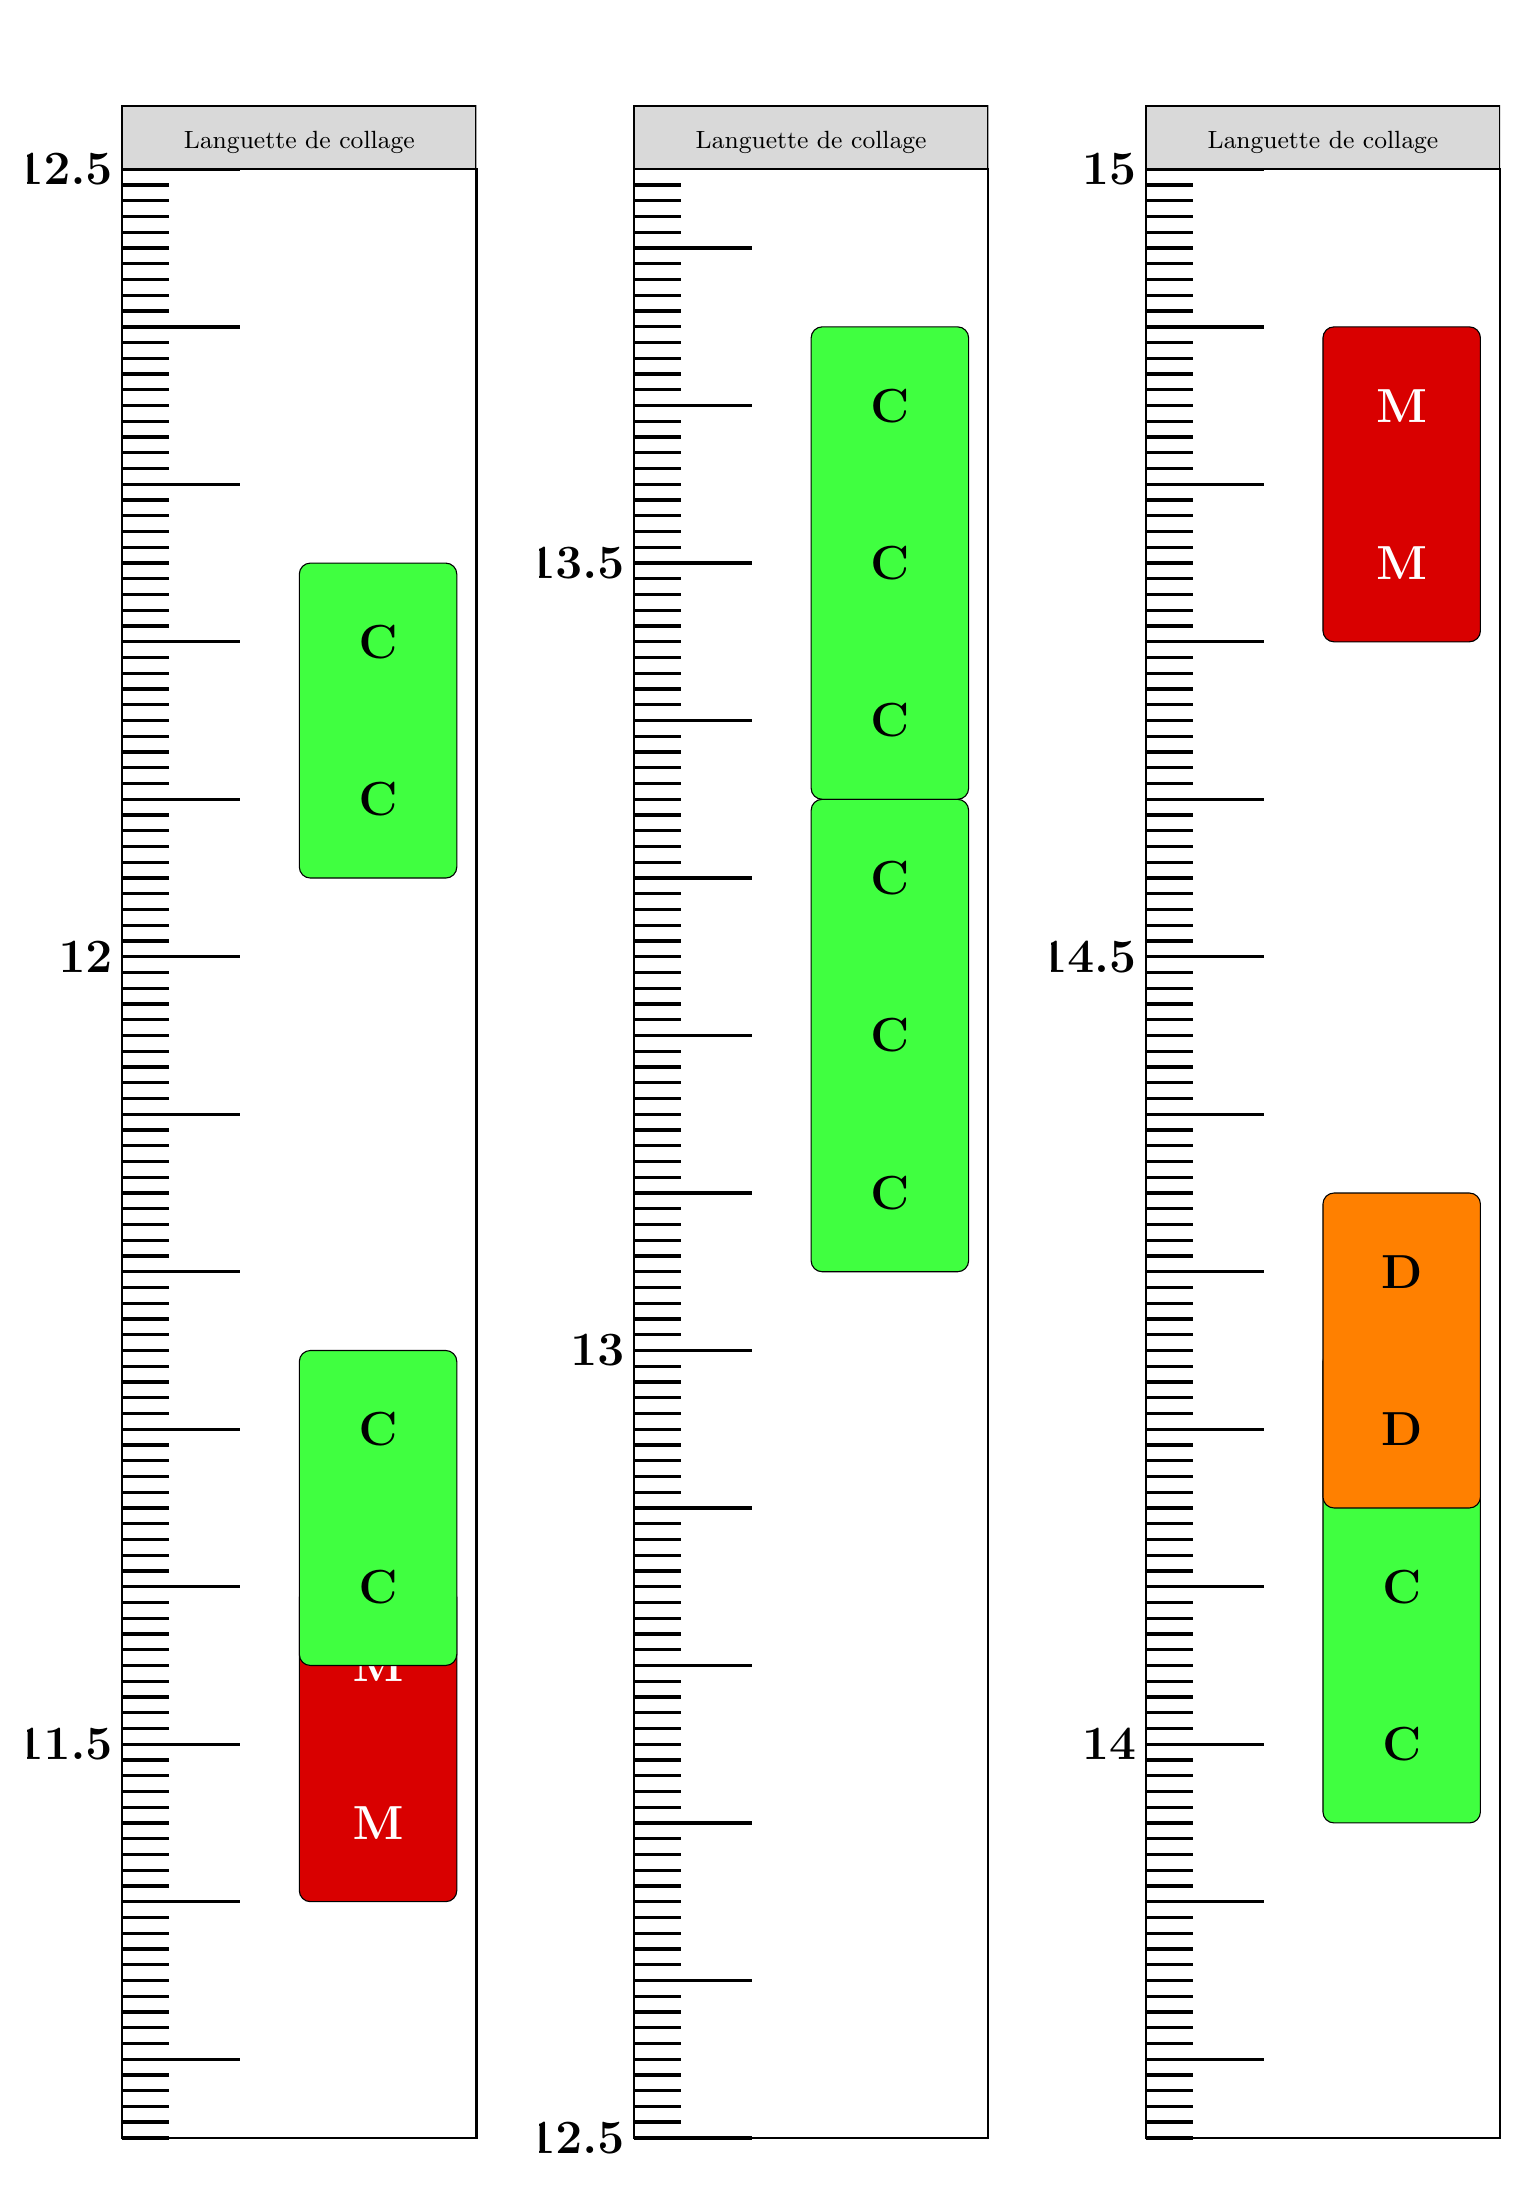
\begin{tikzpicture}[x=1cm, y=1cm,xshift=-1cm]
% Dessin de la première bande
\begin{scope}[shift={(-1,0)}]
    \draw[thick] (0,0) rectangle (\bandwidth, \bandheight);
    \clip (-1.2,-0.5) rectangle (\bandwidth, \bandheight+\languette+1);
    \drawGraduations{0}{12.5}{112.5}{0.5}
\end{scope}

% Dessin de la deuxième bande (avec continuité des nombres)
\begin{scope}[shift={(1*\bandwidth + 1,0)}]
    \draw[thick] (0,0) rectangle (\bandwidth, \bandheight);
    \clip (-1.2,-0.5) rectangle (\bandwidth, \bandheight+\languette+1);
    \drawGraduations{0}{12.5}{125}{0}
\end{scope}

% Dessin de la troisième bande (avec continuité des nombres)
\begin{scope}[shift={(2*\bandwidth + 3,0)}]
    \draw[thick] (0,0) rectangle (\bandwidth, \bandheight);
    \clip (-1.2,-0.5) rectangle (\bandwidth, \bandheight+\languette+1);
    \drawGraduations{0}{12.5}{137.5}{0.5}
\end{scope}

\end{tikzpicture}